\documentclass{article}
\usepackage{listings}
\usepackage{graphicx}
\usepackage{caption}
\usepackage{subcaption}

\DeclareGraphicsExtensions{.png, .jpeg}
% \graphicsPath{{/Users/llaryssa/Documents/Stevens/cs558/hw/hw1latex}}

\begin{document}

\centerline{\sc \large CS 558: Homework Assignment 1}

\centerline{Alana Laryssa Seabra A Santos}
\centerline{\it 2/10/2016}


\section{Gaussian filtering}

The next three sets of images bellow show the input images with gaussian filter applied with three different values of $\sigma$.

\begin{figure}[!h]
  \begin{subfigure}[b]{0.3\textwidth}
  \centering
    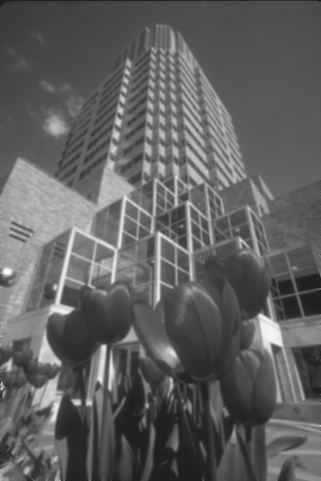
\includegraphics[width=0.85\textwidth]{redsig1}
    \caption{$\sigma = 1$}
    \label{fig:f1}
  \end{subfigure}
  \hfill
  \begin{subfigure}[b]{0.3\textwidth}
    \centering
    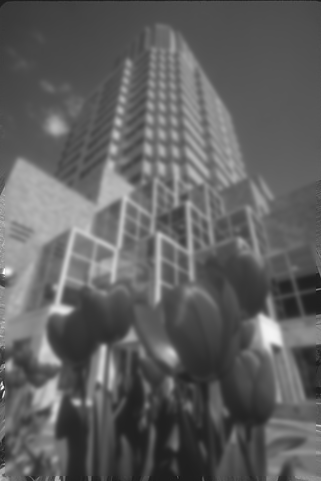
\includegraphics[width=0.85\textwidth]{redsig2}
    \caption{$\sigma = 2$}
    \label{fig:f2}
  \end{subfigure}
   \hfill
  \begin{subfigure}[b]{0.3\textwidth}
    \centering
    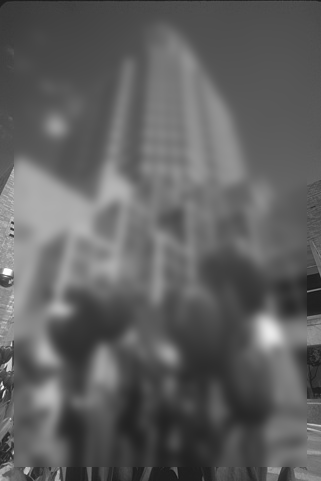
\includegraphics[width=0.85\textwidth]{redsig5}
    \caption{$\sigma = 5$}
    \label{fig:f2}
  \end{subfigure} 
  \caption{Different values of $\sigma$ with red.pgm}
\end{figure}

\begin{figure}[!h]
  \begin{subfigure}{0.3\textwidth}
    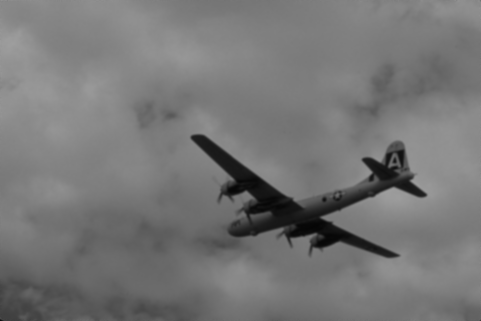
\includegraphics[width=\textwidth]{planesig1}
    \caption{$\sigma = 1$}
    \label{fig:f1}
  \end{subfigure}
  \hfill
  \begin{subfigure}{0.3\textwidth}
    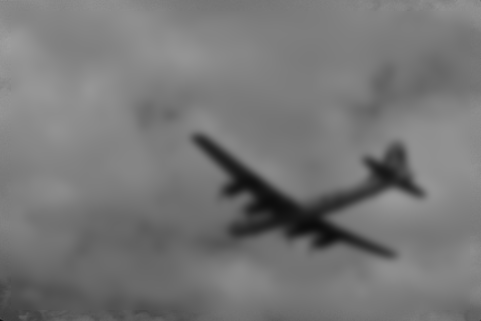
\includegraphics[width=\textwidth]{planesig4}
    \caption{$\sigma = 4$}
    \label{fig:f2}
  \end{subfigure}
   \hfill
  \begin{subfigure}{0.3\textwidth}
    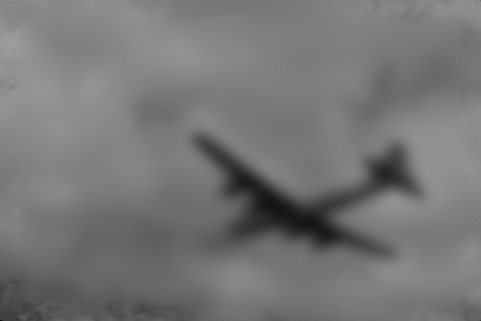
\includegraphics[width=\textwidth]{planesig7}
    \caption{$\sigma = 7$}
    \label{fig:f2}
  \end{subfigure} 
  \caption{Different values of $\sigma$ with plane.pgm}
\end{figure}

\begin{figure}[!h]
  \begin{subfigure}{0.3\textwidth}
    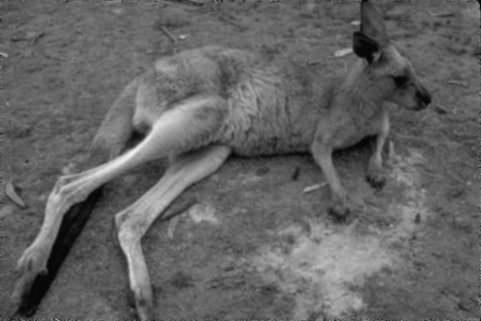
\includegraphics[width=\textwidth]{kangsig1}
    \caption{$\sigma = 1$}
    \label{fig:f1}
  \end{subfigure}
  \hfill
  \begin{subfigure}{0.3\textwidth}
    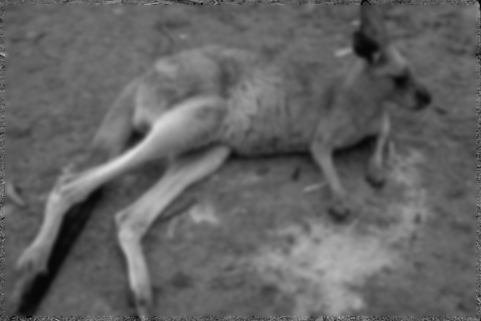
\includegraphics[width=\textwidth]{kangsig2}
    \caption{$\sigma = 2$}
    \label{fig:f2}
  \end{subfigure}
   \hfill
  \begin{subfigure}{0.3\textwidth}
    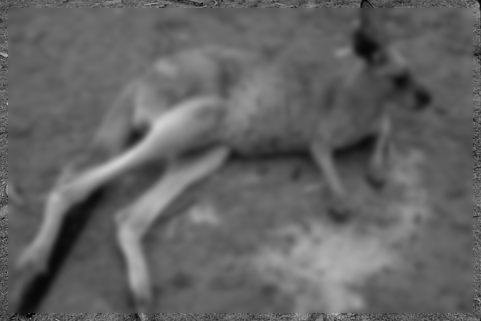
\includegraphics[width=\textwidth]{kangsig3}
    \caption{$\sigma = 3$}
    \label{fig:f2}
  \end{subfigure} 
  \caption{Different values of $\sigma$ with kangaroo.pgm}
\end{figure}

\vspace{.1pc}
\section{Gradient computation}

Bellow I show the best result I got with each one of the input images. All input images for this step were preprocessed with gaussian filter ($\sigma = 1$).


\begin{figure}[!h]
  \begin{subfigure}{0.6\textwidth}
    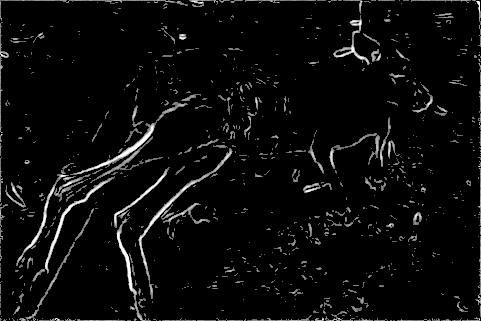
\includegraphics[width=\textwidth]{kangsobel}
    \caption{kangaroo.pgm}
    \label{fig:f1}
  \end{subfigure}
     \hfill
  \begin{subfigure}{0.4\textwidth}
    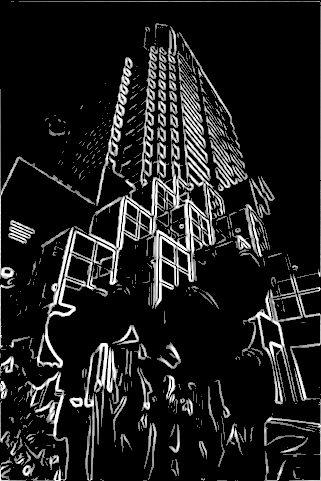
\includegraphics[width=\textwidth]{redsobel}
    \caption{red.pgm}
    \label{fig:f2}
  \end{subfigure}
  \hfill
  
  \begin{subfigure}{0.7\textwidth}
  \centering
    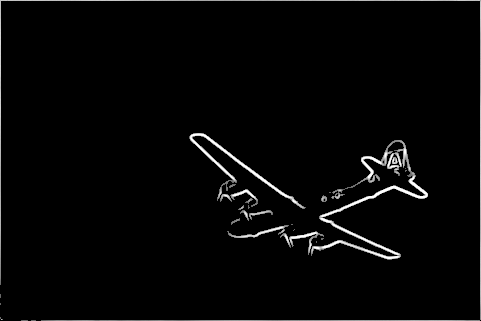
\includegraphics[width=\textwidth]{planesobel}
    \caption{plane.pgm}
    \label{fig:f2}
  \end{subfigure}
 \caption{Gradient strength of the input images}
\end{figure}


\vspace{.1pc}
\section{Non-maximum suppresion}

Bellow are the results when non-maximum suppression technique for edge thinning was applied to each of the images in the previous step. 


\begin{figure}[!h]
  \begin{subfigure}{0.6\textwidth}
    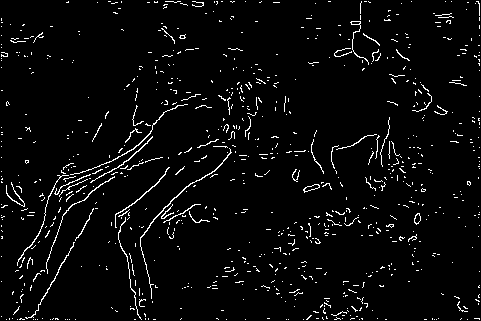
\includegraphics[width=\textwidth]{kangnonmax}
    \caption{kangaroo.pgm}
    \label{fig:f1}
  \end{subfigure}
     \hfill
  \begin{subfigure}{0.4\textwidth}
    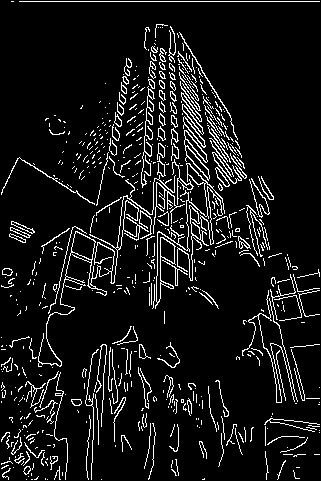
\includegraphics[width=\textwidth]{rednonmax}
    \caption{red.pgm}
    \label{fig:f2}
  \end{subfigure}
  \hfill
  
  \begin{subfigure}{0.7\textwidth}
  \centering
    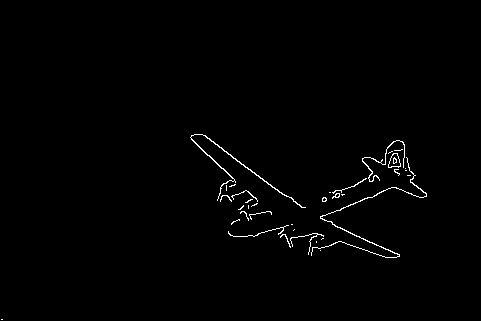
\includegraphics[width=\textwidth]{planenonmax}
    \caption{plane.pgm}
    \label{fig:f2}
  \end{subfigure}
 \caption{Gradient strength of the input images}
\end{figure}



%\begin{figure}[!h]
%\centering
%  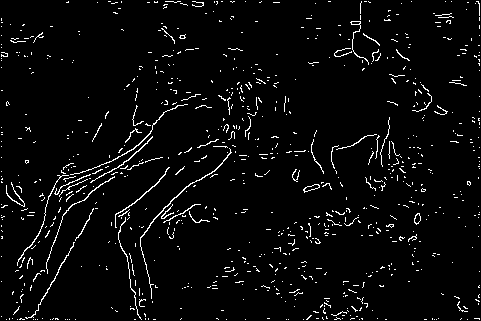
\includegraphics[scale=.5]{kangnonmax}
%\end{figure}
%
%\begin{figure}[!h]
%\centering
%  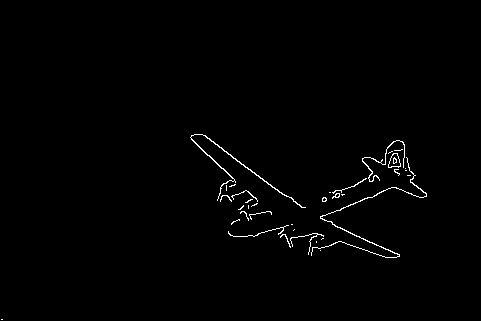
\includegraphics[scale=.5]{planenonmax}
%\end{figure}
%
%\begin{figure}[!h]
%\centering
%  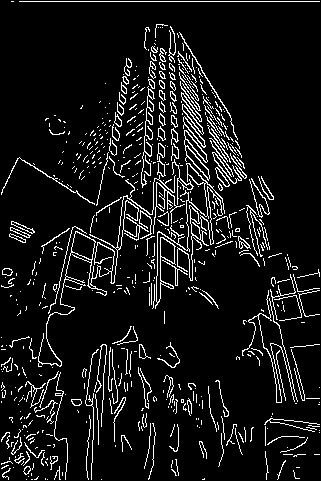
\includegraphics[scale=.4]{rednonmax}
%\end{figure}



\vspace{.1pc}
\section{Matlab code}

Bellow are the Matlab scripts used to generate the presented results

\begin{lstlisting}[language=Matlab]


im = imread('cs558s16_hw1/kangaroo.pgm');
% im = imread('cs558s16_hw1/plane.pgm');
% im = imread('cs558s16_hw1/red.pgm');
% im = [zeros(10,10) ones(10,10); ones(10,10) zeros(10,10)];

im = im2double(im);

% gaussian params
sigma = 1;
% after sobel filter
isedge_thresh = 100;


%% 1. gaussian filter
if sigma ~= 0
    % wingauss = 5;
    % halfgauss = (wingauss-1)/2;
    halfgauss = 3*sigma - 1;

    [x,y] = meshgrid(-halfgauss:halfgauss, -halfgauss:halfgauss);
    G = exp(-(x.^2 + y.^2)/(2*sigma^2));  % no need to compute the const part
    G = G./sum(G(:));  % sum has to be 1

    im1 = filtering(im, G);
else
    im1 = im;
end

%% 2. gradient with sobel filter
Sx = [-1 0 1; -2 0 2; -1 0 1];
Sy = [1 2 1; 0 0 0; -1 -2 -1];

im1x = filtering(im1, Sx);  % has neg values
im1y = filtering(im1, Sy);

strength = sqrt(im1x.^2 + im1y.^2);
direction = atand(im1y./im1x);

strength(im2uint8(strength) < isedge_thresh) = 0;  % binary

%% 3. non-maximum suppression
im2 = nonmaxsup(strength,direction);
edges = im2;
edges(edges > 0) = 1;

function im2 = filtering (im, f)
 % work with images already casted to double
 [s1, s2] = size(f);
 hs1 = (s1-1)/2; hs2 = (s2-1)/2;
 
 im2 = im;  % copy pixels near the borders
%  im2 = zeros(size(im,1),size(im,2));  % fill borders with black
 
 for i = hs1+1 : size(im,1) - hs1
     for j = hs2+1 : size(im,2) - hs2
         im2(i,j) = sum(sum(f.*im(i-hs1:i+hs1, j-hs2:j+hs2)));
     end
 end 
end


function im2 = nonmaxsup(grad, dir)
 % input: gradient, directions
 
 [s1, s2] = size(grad);
 im2 = zeros(size(grad,1), size(grad,2));
 
 for i = 2:s1-1
     for j = 2:s2-1
         if grad(i,j) ~= 0
             x1 = 0; y1 = 0;
             x2 = 0; y2 = 0;
             if dir(i,j) > 67.5 || dir(i,j) <= -67.5 % 90 degrees
                 x1 = -1; y1 = 0;
                 x2 = 1; y2 = 0;
             elseif dir(i,j) <= 67.5 && dir(i,j) > 22.5 % 45 degrees
                 x1 = -1; y1 = 1;
                 x2 = 1; y2 = -1;
             elseif dir(i,j) <= 22.5 && dir(i,j) > -22.5 % 0 degrees
                 x1 = 0; y1 = -1;
                 x2 = 0; y2 = 1;
             elseif dir(i,j) <= -22.5 && dir(i,j) > -67.5 % -45 degrees
                 x1 = -1; y1 = -1;
                 x2 = 1; y2 = 1;
             else
                 disp('wrong');
             end
             
             temp = [grad(i,j) grad(i+x1,j+y1) grad(i+x2,j+y2)];
             if max(temp) == grad(i,j)
                im2(i,j) = grad(i,j);
             end
         end
     end
 end
 
end



\end{lstlisting}

\end{document}


